\documentclass[11pt,a4paper]{article}
\usepackage[utf8]{inputenc}
\usepackage[margin=0.85in]{geometry}
\usepackage{amsmath,amssymb,amsthm}
\usepackage{xcolor}
\usepackage{tcolorbox}
\usepackage{tikz}
\usetikzlibrary{shapes,arrows,positioning,calc,decorations.pathreplacing,patterns}
\usepackage{booktabs}
\usepackage{array}
\usepackage{fancyhdr}
\usepackage{hyperref}
\usepackage{microtype}

% Color Palette Definitions
\definecolor{primarynavy}{RGB}{26, 54, 93}       % #1A365D - Deep Navy
\definecolor{secondaryteal}{RGB}{13, 148, 136}   % #0D9488 - Teal Accent
\definecolor{darkslate}{RGB}{45, 55, 72}        % #2D3748 - Body Text
\definecolor{lightbg}{RGB}{247, 250, 252}        % #F7FAFC - Soft Background
\definecolor{accentblue}{RGB}{49, 130, 206}      % #3182CE - Bright Blue
\definecolor{warmgold}{RGB}{214, 158, 46}        % #D69E2E - Gold Highlight
\definecolor{crimsonred}{RGB}{229, 62, 62}       % #E53E3E - Crimson Alert

\hypersetup{
    colorlinks=true,
    linkcolor=primarynavy,
    citecolor=secondaryteal,
    urlcolor=accentblue,
    pdftitle={Complete Lecture Notes: Metric Spaces and Matrix Spaces},
    pdfauthor={Class Notes}
}

% Page Setup
\pagestyle{fancy}
\fancyhf{}
\fancyhead[L]{\small \textbf{\color{primarynavy}Metric Spaces \& Matrix Spaces (MATMJ53)}}
\fancyhead[R]{\small \textbf{\color{secondaryteal}Lectures by AP Sir}}
\fancyfoot[L]{\small \textcolor{primarynavy}{\href{https://www.sciqb.com}{\textbf{www.sciqb.com}}}}
\fancyfoot[C]{\thepage}
\fancyfoot[R]{\small \textcolor{secondaryteal}{\href{https://www.sciqb.com}{\textbf{SCIQB Platform}}}}
\renewcommand{\headrulewidth}{0.6pt}
\renewcommand{\footrulewidth}{0.4pt}

% Custom TColorBox Environments
\newtcolorbox{defbox}[1]{
    colback=lightbg,
    colframe=primarynavy,
    fonttitle=\bfseries\color{white},
    title={#1},
    boxrule=1pt,
    top=3mm, bottom=3mm, left=4mm, right=4mm
}

\newtcolorbox{formulabox}[1]{
    colback=secondaryteal!8!white,
    colframe=secondaryteal,
    fonttitle=\bfseries\color{white},
    title={#1},
    boxrule=1pt,
    top=3mm, bottom=3mm, left=4mm, right=4mm
}

\newtcolorbox{exbox}[1]{
    colback=white,
    colframe=accentblue,
    fonttitle=\bfseries\color{white},
    title={#1},
    boxrule=1pt,
    top=3mm, bottom=3mm, left=4mm, right=4mm
}

\setlength{\parindent}{0pt}
\setlength{\parskip}{6pt}

\begin{document}

% Title Banner
\begin{center}
    \tcbset{colframe=primarynavy,colback=primarynavy!5!white,arc=0mm}
    \begin{tcolorbox}[sharp corners, boxrule=1.5pt]
        \begin{center}
            {\Large \bfseries \color{primarynavy} COMPLETE MATHEMATICAL LECTURE NOTES ON METRIC SPACES \& MATRIX SPACES}\\[4pt]
            {\large \bfseries \color{secondaryteal} Axioms, Semi-Metrics, Open Spheres, Topological Theorems, Limit Points \& Matrix Norms}\\[6pt]
            {\small \textbf{Course Code:} MATMJ53 \quad|\quad \textbf{Lectures by:} AP Sir \quad|\quad \textbf{Platform:} \href{https://www.sciqb.com}{\color{accentblue}\textbf{www.sciqb.com}}}
        \end{center}
    \end{tcolorbox}
\end{center}

\vspace{0.3cm}

\tableofcontents
\newpage

\section{Module 1: Foundations of Metric Spaces and Semi-Metrics}

A metric space is a mathematical abstraction that formalizes and generalizes the intuitive geometric concept of distance between points in any set.

\subsection{Definition of a Metric Space}

\begin{defbox}{Definition: Metric and Metric Space}
Let $X$ be a non-empty set. A mapping $d: X \times X \to \mathbb{R}$ is called a \textbf{metric} (or distance function) on $X$ if and only if it satisfies the following four fundamental axioms for all elements $x, y, z \in X$:
\begin{enumerate}
    \item[\textbf{[M1]}] \textbf{Non-negativity:}
    \begin{equation}
        d(x, y) \ge 0, \quad \forall x, y \in X
    \end{equation}
    
    \item[\textbf{[M2]}] \textbf{Identity of Indiscernibles (Definiteness):}
    \begin{equation}
        d(x, y) = 0 \iff x = y
    \end{equation}
    
    \item[\textbf{[M3]}] \textbf{Symmetry:}
    \begin{equation}
        d(x, y) = d(y, x), \quad \forall x, y \in X
    \end{equation}
    
    \item[\textbf{[M4]}] \textbf{Triangle Inequality:}
    \begin{equation}
        d(x, y) \le d(x, z) + d(z, y), \quad \forall x, y, z \in X
    \end{equation}
\end{enumerate}
If $d$ is a metric on $X$, then the ordered pair $(X, d)$ is called a \textbf{Metric Space}, and the non-negative real number $d(x, y)$ is called the \textbf{distance between $x$ and $y$}.
\end{defbox}

\begin{center}
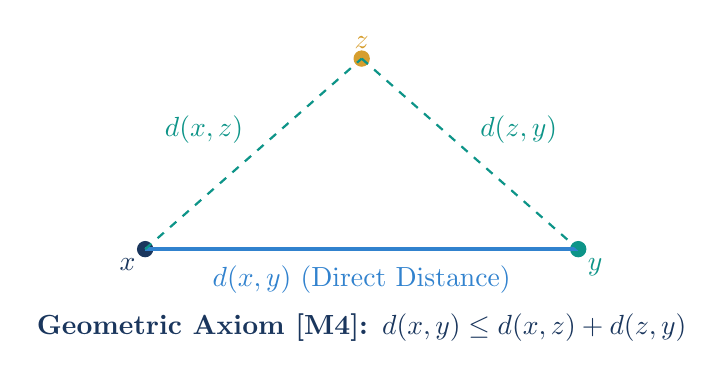
\begin{tikzpicture}[scale=1.1]
    \filldraw[primarynavy] (0,0) circle (2.5pt) node[below left] {$x$};
    \filldraw[secondaryteal] (5,0) circle (2.5pt) node[below right] {$y$};
    \filldraw[warmgold] (2.5,2.2) circle (2.5pt) node[above] {$z$};
    
    \draw[ultra thick,accentblue] (0,0) -- (5,0) node[midway,below=2pt] {$d(x,y)$ (Direct Distance)};
    \draw[thick,dashed,secondaryteal] (0,0) -- (2.5,2.2) node[midway,above left] {$d(x,z)$};
    \draw[thick,dashed,secondaryteal] (2.5,2.2) -- (5,0) node[midway,above right] {$d(z,y)$};
    
    \node[primarynavy,font=\bfseries] at (2.5,-0.9) {Geometric Axiom [M4]: $d(x,y) \le d(x,z) + d(z,y)$};
\end{tikzpicture}
\end{center}

\subsection{Semi-Metric (Pseudo-Metric)}

\begin{defbox}{Definition: Semi-Metric / Pseudo-Metric}
A mapping $d: X \times X \to \mathbb{R}$ is called a \textbf{semi-metric} (or \textbf{pseudo-metric}) if and only if it satisfies:
\begin{enumerate}
    \item[\textbf{[M1]}] $d(x, y) \ge 0, \quad \forall x, y \in X$.
    \item[\textbf{[M2']}] $d(x, x) = 0, \quad \forall x \in X$ (Note: $d(x, y) = 0$ does \textbf{not} require $x = y$).
    \item[\textbf{[M3]}] $d(x, y) = d(y, x), \quad \forall x, y \in X$.
    \item[\textbf{[M4]}] $d(x, y) \le d(x, z) + d(z, y), \quad \forall x, y, z \in X$.
\end{enumerate}
\textbf{Remark:} Every metric is a semi-metric, but a semi-metric is generally \textbf{not} a metric because distinct points may have zero distance.
\end{defbox}

\begin{exbox}{Example: A Semi-Metric that is NOT a Metric}
\textbf{Question:} Consider the mapping $d: \mathbb{R} \times \mathbb{R} \to \mathbb{R}$ defined by:
\begin{equation}
    d(x, y) = |x^2 - y^2|, \quad \forall x, y \in \mathbb{R}
\end{equation}
Show that $d$ is a semi-metric on $\mathbb{R}$, but is \textbf{not} a metric.

\textbf{Verification of Axioms:}
\begin{enumerate}
    \item \textbf{[M1] Non-negativity:} Since absolute value is always non-negative, $d(x, y) = |x^2 - y^2| \ge 0, \; \forall x, y \in \mathbb{R}$.
    
    \item \textbf{[M3] Symmetry:} $d(x, y) = |x^2 - y^2| = |-(y^2 - x^2)| = |y^2 - x^2| = d(y, x)$.
    
    \item \textbf{[M4] Triangle Inequality:} For any $x, y, z \in \mathbb{R}$:
    \begin{align}
        d(x, y) &= |x^2 - y^2| = |(x^2 - z^2) + (z^2 - y^2)| \notag \\
        &\le |x^2 - z^2| + |z^2 - y^2| = d(x, z) + d(z, y)
    \end{align}
    
    \item \textbf{[M2] Failure of Indiscernibles:}
    \begin{align}
        d(x, y) = 0 &\iff |x^2 - y^2| = 0 \iff x^2 = y^2 \notag \\
        &\iff x = y \quad \text{or} \quad x = -y
    \end{align}
    For instance, choose $x = 2$ and $y = -2$:
    $$d(2, -2) = |2^2 - (-2)^2| = |4 - 4| = 0$$
    However, $2 \neq -2$. Therefore, condition $[M2]$ fails.
\end{enumerate}
\textbf{Conclusion:} $d(x, y) = |x^2 - y^2|$ is a \textbf{semi-metric} (pseudo-metric), but \textbf{not a metric} on $\mathbb{R}$. \qed
\end{exbox}

\newpage

\subsection{Standard Metrics on Euclidean Spaces}

\begin{formulabox}{Standard Metrics on $\mathbb{R}^2$}
Let $x = (x_1, y_1)$ and $y = (x_2, y_2)$ be points in $\mathbb{R}^2$.
\begin{enumerate}
    \item \textbf{Euclidean Metric ($d_2$):}
    \begin{equation}
        d_2(x, y) = \sqrt{(x_2 - x_1)^2 + (y_2 - y_1)^2}
    \end{equation}
    
    \item \textbf{Taxicab / Manhattan Metric ($d_1$):}
    \begin{equation}
        d_1(x, y) = |x_1 - x_2| + |y_1 - y_2|
    \end{equation}
    
    \item \textbf{Maximum / Chebyshev Metric ($d_\infty$):}
    \begin{equation}
        d_\infty(x, y) = \max\left( |x_1 - x_2|, |y_1 - y_2| \right)
    \end{equation}
\end{enumerate}
\end{formulabox}

\subsection{Discrete Metric Space}

\begin{defbox}{Definition: Discrete Metric Space}
Let $X$ be any arbitrary non-empty set. The \textbf{discrete metric} on $X$ is defined as:
\begin{equation}
    d(x, y) = 0 \quad \text{if } x = y, \qquad \text{and} \qquad d(x, y) = 1 \quad \text{if } x \neq y
\end{equation}
The pair $(X, d)$ is called a \textbf{Discrete Metric Space}. In this space, every single point is isolated at a distance of 1 from every other point.
\end{defbox}

\subsection{Matrix Spaces as Metric Spaces}

Let $M_{m \times n}(\mathbb{R})$ denote the vector space of all $m \times n$ real matrices.

\begin{defbox}{Definition: Frobenius Metric on Matrix Space}
For any matrices $A, B \in M_{m \times n}(\mathbb{R})$, the \textbf{Frobenius distance} is defined by:
\begin{equation}
    d_F(A, B) = \|A - B\|_F = \sqrt{\sum_{i=1}^m \sum_{j=1}^n (a_{ij} - b_{ij})^2} = \sqrt{\operatorname{Tr}\left((A-B)^T(A-B)\right)}
\end{equation}
\textbf{Properties:}
\begin{itemize}
    \item $d_F(A, B) \ge 0$ and $d_F(A, B) = 0 \iff A = B$.
    \item $d_F(A, B) = d_F(B, A)$.
    \item $d_F(A, B) \le d_F(A, C) + d_F(C, B)$ (follows from Cauchy-Schwarz on matrix trace).
    \item $(M_{m \times n}(\mathbb{R}), d_F)$ is isometrically isomorphic to the Euclidean space $(\mathbb{R}^{mn}, d_2)$ and is therefore a \textbf{complete metric space}.
\end{itemize}
\end{defbox}

\newpage

\section{Module 2: Open Spheres, Neighborhoods, and Interior Points}

\subsection{Open Spheres (Open Balls)}

\begin{defbox}{Definition: Open Sphere / Open Ball}
Let $(X, d)$ be a metric space, $x_0 \in X$, and $r > 0$ be a positive real number. The \textbf{open sphere} (or open ball) centered at $x_0$ of radius $r$ is the subset:
\begin{equation}
    S_r(x_0) = B(x_0, r) = \{ x \in X \mid d(x, x_0) < r \}
\end{equation}
The \textbf{closed sphere} centered at $x_0$ of radius $r$ is:
\begin{equation}
    \bar{S}_r(x_0) = \bar{B}(x_0, r) = \{ x \in X \mid d(x, x_0) \le r \}
\end{equation}
\end{defbox}

\subsection{Geometric Shapes of Open Spheres in Different Metrics}

\begin{exbox}{Examples: Open Spheres with $x_0 = (0,0)$ and $r = 1$}
\begin{enumerate}
    \item \textbf{Usual Metric on $\mathbb{R}$ with $x_0 = 0, r = 1$:}
    $$S_1(0) = \{ x \in \mathbb{R} \mid d(x, 0) < 1 \} = \{ x \in \mathbb{R} \mid |x| < 1 \} = \mathbf{(-1, 1)} \quad \text{(Open Interval)}$$
    
    \item \textbf{Euclidean Metric $(\mathbb{R}^2, d_2)$ with $x_0 = (0,0), r = 1$:}
    $$S_1(0,0) = \{ (x, y) \in \mathbb{R}^2 \mid \sqrt{x^2 + y^2} < 1 \} = \{ (x, y) \mid \mathbf{x^2 + y^2 < 1} \} \quad \text{(Circular Disk)}$$
    
    \item \textbf{Taxicab Metric $(\mathbb{R}^2, d_1)$ with $x_0 = (0,0), r = 1$:}
    $$S_1(0,0) = \{ (x, y) \in \mathbb{R}^2 \mid \mathbf{|x| + |y| < 1} \} \quad \text{(Rotated Square / Diamond)}$$
    
    \item \textbf{Maximum Metric $(\mathbb{R}^2, d_\infty)$ with $x_0 = (0,0), r = 1$:}
    $$S_1(0,0) = \{ (x, y) \in \mathbb{R}^2 \mid \max(|x|, |y|) < 1 \} = \mathbf{(-1, 1) \times (-1, 1)} \quad \text{(Axis-aligned Square)}$$
    
    \item \textbf{Discrete Metric Space $(X, d)$:}
    $$S_r(x_0) = \{x_0\} \quad \text{if } r \le 1, \qquad \text{and} \qquad S_r(x_0) = X \quad \text{if } r > 1$$
\end{enumerate}
\end{exbox}

\begin{center}
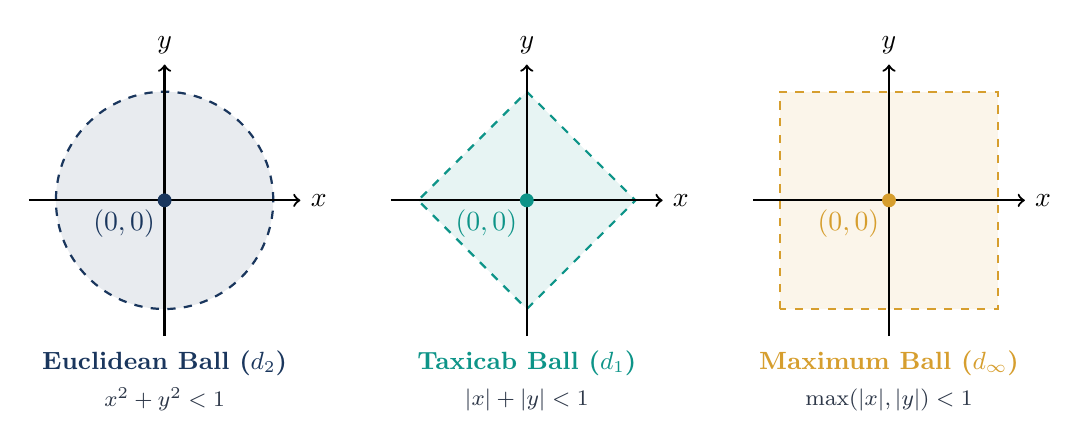
\begin{tikzpicture}[scale=1.15]
    % Euclidean ball (circle)
    \draw[dashed,thick,primarynavy,fill=primarynavy!10] (-4,0) circle (1.2cm);
    \draw[->,thick] (-5.5,0) -- (-2.5,0) node[right] {$x$};
    \draw[->,thick] (-4,-1.5) -- (-4,1.5) node[above] {$y$};
    \filldraw[primarynavy] (-4,0) circle (2pt) node[below left] {$(0,0)$};
    \node[primarynavy,font=\bfseries\small] at (-4,-1.8) {Euclidean Ball ($d_2$)};
    \node[darkslate,font=\footnotesize] at (-4,-2.2) {$x^2 + y^2 < 1$};

    % Taxicab ball (diamond)
    \draw[dashed,thick,secondaryteal,fill=secondaryteal!10] (0,1.2) -- (1.2,0) -- (0,-1.2) -- (-1.2,0) -- cycle;
    \draw[->,thick] (-1.5,0) -- (1.5,0) node[right] {$x$};
    \draw[->,thick] (0,-1.5) -- (0,1.5) node[above] {$y$};
    \filldraw[secondaryteal] (0,0) circle (2pt) node[below left] {$(0,0)$};
    \node[secondaryteal,font=\bfseries\small] at (0,-1.8) {Taxicab Ball ($d_1$)};
    \node[darkslate,font=\footnotesize] at (0,-2.2) {$|x| + |y| < 1$};

    % Maximum metric ball (square)
    \draw[dashed,thick,warmgold,fill=warmgold!10] (2.8,-1.2) rectangle (5.2,1.2);
    \draw[->,thick] (2.5,0) -- (5.5,0) node[right] {$x$};
    \draw[->,thick] (4,-1.5) -- (4,1.5) node[above] {$y$};
    \filldraw[warmgold] (4,0) circle (2pt) node[below left] {$(0,0)$};
    \node[warmgold,font=\bfseries\small] at (4,-1.8) {Maximum Ball ($d_\infty$)};
    \node[darkslate,font=\footnotesize] at (4,-2.2) {$\max(|x|, |y|) < 1$};
\end{tikzpicture}
\end{center}

\begin{center}
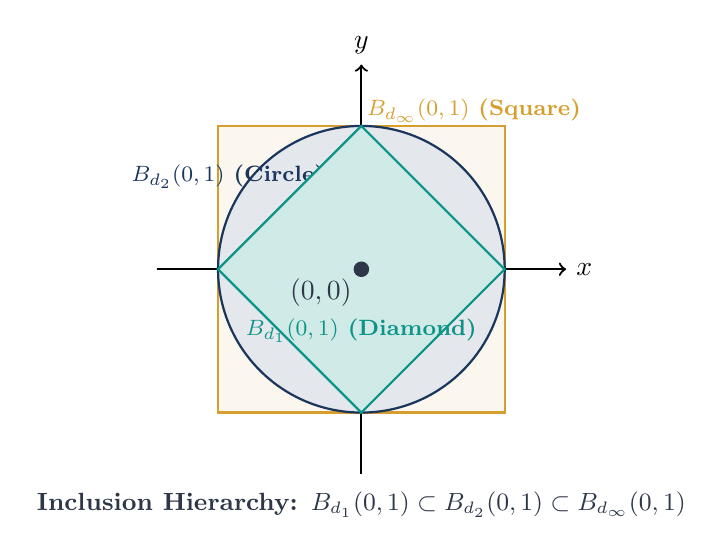
\begin{tikzpicture}[scale=1.3]
    % Overlay diagram of all 3 balls centered at (0,0)
    \draw[->,thick] (-2,0) -- (2,0) node[right] {$x$};
    \draw[->,thick] (0,-2) -- (0,2) node[above] {$y$};
    
    % Chebyshev ball d_infinity (Square)
    \draw[thick,warmgold,fill=warmgold!8] (-1.4,-1.4) rectangle (1.4,1.4);
    \node[warmgold,font=\bfseries\footnotesize] at (1.1,1.55) {$B_{d_\infty}(0,1)$ (Square)};
    
    % Euclidean ball d_2 (Circle)
    \draw[thick,primarynavy,fill=primarynavy!12] (0,0) circle (1.4cm);
    \node[primarynavy,font=\bfseries\footnotesize] at (-1.3,0.9) {$B_{d_2}(0,1)$ (Circle)};
    
    % Taxicab ball d_1 (Diamond)
    \draw[thick,secondaryteal,fill=secondaryteal!20] (0,1.4) -- (1.4,0) -- (0,-1.4) -- (-1.4,0) -- cycle;
    \node[secondaryteal,font=\bfseries\footnotesize] at (0,-0.6) {$B_{d_1}(0,1)$ (Diamond)};
    
    \filldraw[darkslate] (0,0) circle (2pt) node[below left] {$(0,0)$};
    \node[darkslate,font=\bfseries\small] at (0,-2.3) {Inclusion Hierarchy: $B_{d_1}(0,1) \subset B_{d_2}(0,1) \subset B_{d_\infty}(0,1)$};
\end{tikzpicture}
\end{center}

\newpage

\subsection{Neighborhoods and Interior Points}

\begin{defbox}{Definitions: Neighborhood and Open Neighborhood}
Let $(X, d)$ be a metric space and $x \in X$.
\begin{itemize}
    \item A subset $N \subseteq X$ is called a \textbf{neighborhood of $x$} if and only if there exists an open sphere $S_r(x)$ centered at $x$ with radius $r > 0$ such that:
    \begin{equation}
        S_r(x) \subseteq N
    \end{equation}
    \item If the neighborhood $N$ is itself an open set, it is called an \textbf{open neighborhood} of $x$.
\end{itemize}
\end{defbox}

\begin{defbox}{Definitions: Interior Point and Interior of a Set}
Let $G$ be a subset of a metric space $(X, d)$.
\begin{itemize}
    \item A point $x \in G$ is called an \textbf{interior point} of $G$ if and only if there exists an open sphere $S_r(x)$ with $r > 0$ such that:
    \begin{equation}
        S_r(x) \subseteq G
    \end{equation}
    \item The set of all interior points of $G$ is called the \textbf{interior of $G$}, denoted by $G^\circ$ or $\operatorname{Int}(G)$.
    \item \textbf{Theorem:} A subset $G$ is an \textbf{open set} if and only if every point of $G$ is an interior point of $G$ ($G = G^\circ$).
\end{itemize}
\end{defbox}

\begin{center}
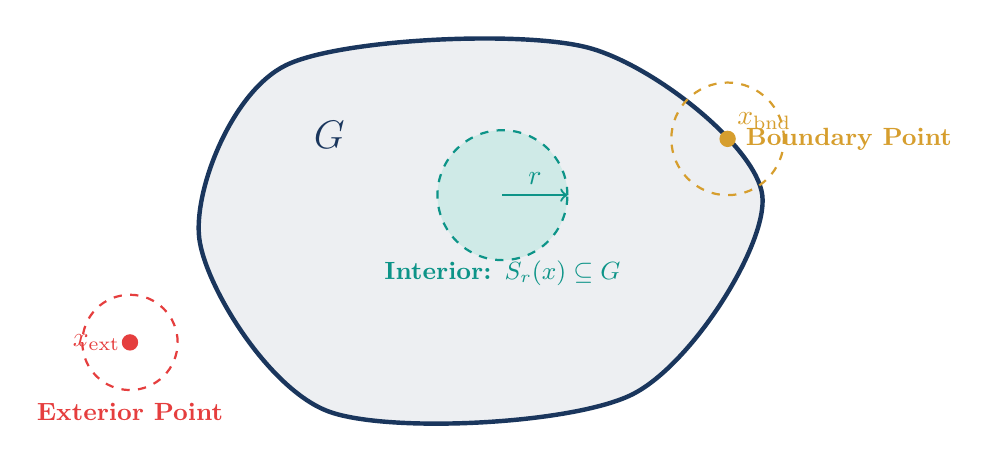
\begin{tikzpicture}[scale=1.1]
    % Topological set G boundary
    \draw[ultra thick,primarynavy,fill=primarynavy!8,smooth cycle] 
        plot coordinates {(-3,0) (-2,2) (1.5,2.2) (3.5,0.5) (2,-1.8) (-1.5,-2)};
    \node[primarynavy,font=\Large\bfseries] at (-1.5,1.2) {$G$};

    % Interior point x_int
    \filldraw[secondaryteal] (0.5,0.5) circle (2.5pt) node[below right] {$x_{\text{int}}$};
    \draw[dashed,thick,secondaryteal,fill=secondaryteal!20] (0.5,0.5) circle (0.75cm);
    \draw[->,thick,secondaryteal] (0.5,0.5) -- (1.25,0.5) node[midway,above] {$r$};
    \node[secondaryteal,font=\bfseries\small] at (0.5,-0.4) {Interior: $S_r(x) \subseteq G$};

    % Boundary point x_bnd
    \filldraw[warmgold] (3.1,1.15) circle (2.5pt) node[above right] {$x_{\text{bnd}}$};
    \draw[dashed,thick,warmgold] (3.1,1.15) circle (0.65cm);
    \node[warmgold,font=\bfseries\small] at (4.5,1.15) {Boundary Point};

    % Exterior point x_ext
    \filldraw[crimsonred] (-3.8,-1.2) circle (2.5pt) node[left] {$x_{\text{ext}}$};
    \draw[dashed,thick,crimsonred] (-3.8,-1.2) circle (0.55cm);
    \node[crimsonred,font=\bfseries\small] at (-3.8,-2.0) {Exterior Point};
\end{tikzpicture}
\end{center}

\newpage

\section{Module 3: Topology of Open Sets and Fundamental Theorems}

\subsection{Open Sets in a Metric Space}

\begin{defbox}{Definition: Open Set}
A subset $G$ of a metric space $(X, d)$ is called an \textbf{open set} if and only if for each point $x \in G$, there exists a real number $r > 0$ such that:
\begin{equation}
    S_r(x) \subseteq G
\end{equation}
\end{defbox}

\subsection{Fundamental Theorems on Open Sets with Complete Proofs}

\begin{exbox}{Theorem 1: The Empty Set $\emptyset$ and Full Space $X$ are Open}
\textbf{Theorem:} In any metric space $(X, d)$, the empty set $\emptyset$ and the full space $X$ are open sets.

\textbf{Proof:}
\begin{enumerate}
    \item \textbf{For the empty set $\emptyset$:} A set $G$ is open if every $x \in G$ has an open ball contained in $G$. Since $\emptyset$ contains no elements, the condition holds vacuously. Thus, $\emptyset$ is open.
    \item \textbf{For the full space $X$:} Let $x \in X$ be arbitrary. Choose any radius $r > 0$. By definition, the open sphere $S_r(x) = \{y \in X \mid d(y, x) < r\} \subseteq X$. Hence every point of $X$ is an interior point of $X$, so $X$ is open. \qed
\end{enumerate}
\end{exbox}

\begin{exbox}{Theorem 2: Every Open Sphere is an Open Set}
\textbf{Theorem:} In a metric space $(X, d)$, every open sphere $S_r(x_0)$ is an open set.

\textbf{Proof:}
\begin{enumerate}
    \item Let $S_r(x_0)$ be an open sphere centered at $x_0 \in X$ with radius $r > 0$.
    \item Let $x$ be an arbitrary point in $S_r(x_0)$. Then by definition:
    \begin{equation}
        d(x, x_0) < r \implies r - d(x, x_0) > 0
    \end{equation}
    \item Choose the radius $\rho = r - d(x, x_0) > 0$.
    \item \textbf{Claim:} $S_\rho(x) \subseteq S_r(x_0)$.
    \item To prove the claim, let $y \in S_\rho(x)$. Then $d(y, x) < \rho$.
    \item By the triangle inequality $[M4]$ on the metric $d$:
    \begin{align}
        d(y, x_0) &\le d(y, x) + d(x, x_0) \notag \\
        &< \rho + d(x, x_0) \notag \\
        &= (r - d(x, x_0)) + d(x, x_0) \notag \\
        &= r
    \end{align}
    \item Since $d(y, x_0) < r$, it follows that $y \in S_r(x_0)$.
    \item Therefore, $S_\rho(x) \subseteq S_r(x_0)$.
    \item Since $x \in S_r(x_0)$ was arbitrary, every point in $S_r(x_0)$ is an interior point.
    \item Hence, $S_r(x_0)$ is an \textbf{open set}. \qed
\end{enumerate}
\end{exbox}

\begin{center}
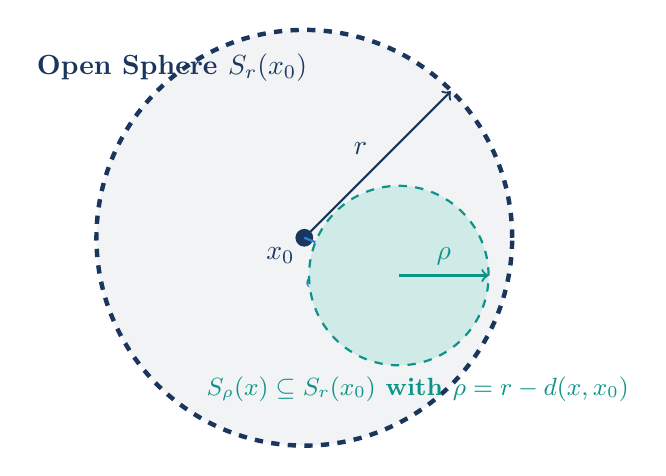
\begin{tikzpicture}[scale=1.2]
    % Outer open sphere S_r(x_0)
    \draw[dashed,ultra thick,primarynavy,fill=primarynavy!6] (0,0) circle (2.2cm);
    \filldraw[primarynavy] (0,0) circle (2.5pt) node[below left] {$x_0$};
    \draw[->,thick,primarynavy] (0,0) -- (1.55,1.55) node[midway,above left] {$r$};
    \node[primarynavy,font=\bfseries] at (-1.4,1.8) {Open Sphere $S_r(x_0)$};

    % Point x in S_r(x_0)
    \filldraw[secondaryteal] (1.0,-0.4) circle (2.5pt) node[below left] {$x$};
    \draw[thick,accentblue] (0,0) -- (1.0,-0.4) node[midway,below] {$d(x,x_0)$};

    % Inscribed open sphere S_rho(x)
    \draw[dashed,thick,secondaryteal,fill=secondaryteal!20] (1.0,-0.4) circle (0.95cm);
    \draw[->,thick,secondaryteal] (1.0,-0.4) -- (1.95,-0.4) node[midway,above] {$\rho$};
    \node[secondaryteal,font=\bfseries\small] at (1.2,-1.6) {$S_\rho(x) \subseteq S_r(x_0)$ with $\rho = r - d(x,x_0)$};
\end{tikzpicture}
\end{center}

\newpage

\begin{exbox}{Theorem 3: Arbitrary Union of Open Sets is Open}
\textbf{Theorem:} In a metric space $(X, d)$, the union of an arbitrary collection of open sets is an open set.

\textbf{Proof:}
\begin{enumerate}
    \item Let $\{G_\lambda \mid \lambda \in \Lambda\}$ be an arbitrary collection of open sets in $(X, d)$, where $\Lambda$ is an arbitrary index set.
    \item Let $G = \bigcup_{\lambda \in \Lambda} G_\lambda$.
    \item If $G = \emptyset$, then $G$ is open by Theorem 1.
    \item If $G \neq \emptyset$, let $x \in G$.
    \item By definition of union, $x \in G_{\lambda_0}$ for some specific index $\lambda_0 \in \Lambda$.
    \item Since $G_{\lambda_0}$ is an open set, there exists a radius $r > 0$ such that:
    \begin{equation}
        S_r(x) \subseteq G_{\lambda_0}
    \end{equation}
    \item Since $G_{\lambda_0} \subseteq \bigcup_{\lambda \in \Lambda} G_\lambda = G$, it follows that:
    \begin{equation}
        S_r(x) \subseteq G
    \end{equation}
    \item Since $x \in G$ was chosen arbitrarily, every point of $G$ is an interior point.
    \item Hence, $G = \bigcup_{\lambda \in \Lambda} G_\lambda$ is an \textbf{open set}. \qed
\end{enumerate}
\end{exbox}

\begin{exbox}{Theorem 4: Finite Intersection of Open Sets is Open}
\textbf{Theorem:} In a metric space $(X, d)$, the intersection of a finite number of open sets is an open set.

\textbf{Proof:}
\begin{enumerate}
    \item Let $G_1, G_2, \dots, G_n$ be a finite collection of open sets in $(X, d)$.
    \item Let $G = \bigcap_{i=1}^n G_i$.
    \item If $G = \emptyset$, then $G$ is open by Theorem 1.
    \item If $G \neq \emptyset$, let $x \in G$.
    \item By definition of intersection, $x \in G_i$ for every $i \in \{1, 2, \dots, n\}$.
    \item Since each $G_i$ is open, there exist positive real radii $r_1, r_2, \dots, r_n > 0$ such that:
    \begin{equation}
        S_{r_i}(x) \subseteq G_i, \quad \forall i \in \{1, 2, \dots, n\}
    \end{equation}
    \item Define $r = \min \{r_1, r_2, \dots, r_n\}$. Since it is the minimum of a \textbf{finite} collection of strictly positive numbers, $r > 0$.
    \item Since $r \le r_i$ for each $i$, we have $S_r(x) \subseteq S_{r_i}(x) \subseteq G_i$ for all $i = 1, 2, \dots, n$.
    \item Therefore:
    \begin{equation}
        S_r(x) \subseteq \bigcap_{i=1}^n G_i = G
    \end{equation}
    \item Since $x \in G$ was arbitrary, $G = \bigcap_{i=1}^n G_i$ is an \textbf{open set}. \qed
\end{enumerate}
\end{exbox}

\begin{formulabox}{Important Counterexample: Infinite Intersection of Open Sets May NOT be Open}
In $(\mathbb{R}, |\cdot|)$, consider the infinite family of open intervals:
\begin{equation}
    G_n = \left( -\frac{1}{n}, \frac{1}{n} \right), \quad n \in \mathbb{N}
\end{equation}
Each $G_n$ is an open set in $\mathbb{R}$. However, their infinite intersection is:
\begin{equation}
    \bigcap_{n=1}^\infty G_n = \bigcap_{n=1}^\infty \left( -\frac{1}{n}, \frac{1}{n} \right) = \{0\}
\end{equation}
The singleton set $\{0\}$ is a \textbf{closed set} and is \textbf{not open} in $(\mathbb{R}, |\cdot|)$, because for any $r > 0$, the open ball $S_r(0) = (-r, r) \not\subseteq \{0\}$.
\end{formulabox}

\begin{center}
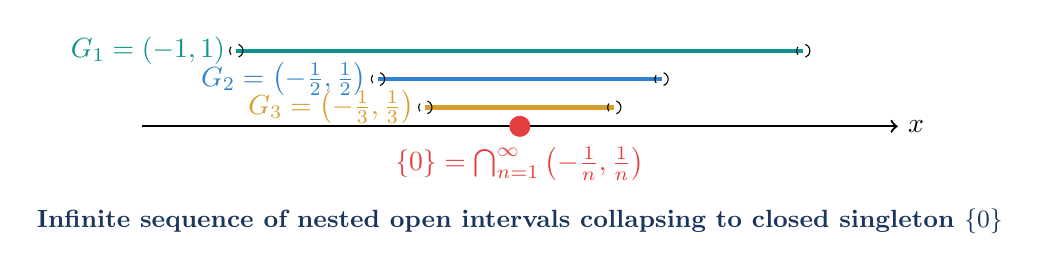
\begin{tikzpicture}[scale=1.2]
    \draw[->,thick] (-4,0) -- (4,0) node[right] {$x$};
    \filldraw[crimsonred] (0,0) circle (3pt) node[below=4pt] {$\{0\} = \bigcap_{n=1}^\infty \left(-\frac{1}{n}, \frac{1}{n}\right)$};
    
    \draw[ultra thick,secondaryteal] (-3,0.8) node[left] {$G_1 = (-1, 1)$} -- (3,0.8);
    \draw[dashed] (-3,0.8) circle (2pt); \draw[dashed] (3,0.8) circle (2pt);

    \draw[ultra thick,accentblue] (-1.5,0.5) node[left] {$G_2 = \left(-\frac{1}{2}, \frac{1}{2}\right)$} -- (1.5,0.5);
    \draw[dashed] (-1.5,0.5) circle (2pt); \draw[dashed] (1.5,0.5) circle (2pt);

    \draw[ultra thick,warmgold] (-1.0,0.2) node[left] {$G_3 = \left(-\frac{1}{3}, \frac{1}{3}\right)$} -- (1.0,0.2);
    \draw[dashed] (-1.0,0.2) circle (2pt); \draw[dashed] (1.0,0.2) circle (2pt);

    \node[primarynavy,font=\bfseries\small] at (0,-1.0) {Infinite sequence of nested open intervals collapsing to closed singleton $\{0\}$};
\end{tikzpicture}
\end{center}

\newpage

\section{Module 4: Limit Points, Derived Sets, and Closed Sets}

\subsection{Limit Points (Accumulation Points)}

\begin{defbox}{Definition: Limit Point of a Set}
Let $(X, d)$ be a metric space and $A \subseteq X$. A point $p \in X$ is called a \textbf{limit point} (or \textbf{accumulation point} / cluster point) of $A$ if and only if every neighborhood $N_p$ of $p$ contains at least one point of $A$ different from $p$:
\begin{equation}
    \left( N_p \setminus \{p\} \right) \cap A \neq \emptyset
\end{equation}
Equivalently, for every $r > 0$:
\begin{equation}
    \left( S_r(p) \setminus \{p\} \right) \cap A \neq \emptyset
\end{equation}
\end{defbox}

\subsection{Derived Sets and Examples}

\begin{defbox}{Definition: Derived Set $A'$}
The set of all limit points of a subset $A$ is called the \textbf{derived set} of $A$, denoted by $A'$ or $d(A)$.
\end{defbox}

\begin{exbox}{Solved Examples on Derived Sets}
\begin{enumerate}
    \item \textbf{Harmonic Sequence Set in $(\mathbb{R}, |\cdot|)$:}
    Let $A = \left\{ 1, \frac{1}{2}, \frac{1}{3}, \dots, \frac{1}{n}, \dots \right\}$.
    The only accumulation point is $0$, because for every $\varepsilon > 0$, $(-\varepsilon, \varepsilon) \cap A$ contains infinitely many terms $\frac{1}{n}$. None of the elements $\frac{1}{n} \in A$ are limit points.
    $$\mathbf{A' = \{0\}}$$
    
    \item \textbf{Open Interval in $(\mathbb{R}, |\cdot|)$:}
    Let $A = (0, 1)$. Every point in $(0, 1)$ as well as the endpoints $0$ and $1$ are limit points:
    $$\mathbf{A' = [0, 1]}$$
    
    \item \textbf{Topologist's Sine Curve in $\mathbb{R}^2$:}
    Consider the subset $A = \left\{ (x, y) \in \mathbb{R}^2 \mid y = \sin\left(\frac{1}{x}\right), \; x > 0 \right\}$.
    As $x \to 0^+$, $\sin(1/x)$ oscillates between $-1$ and $+1$ infinitely often.
    The derived set $A'$ contains the curve itself plus the entire vertical segment on the $y$-axis:
    $$\mathbf{A' = A \cup \left( \{0\} \times [-1, 1] \right)}$$
\end{enumerate}
\end{exbox}

\begin{center}
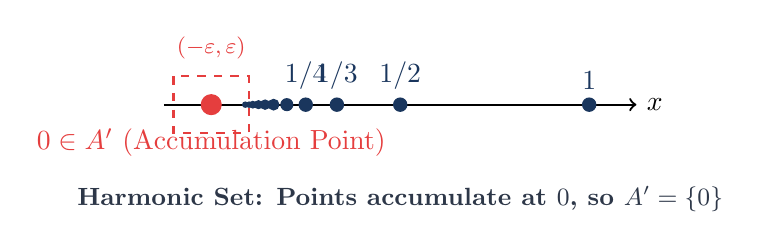
\begin{tikzpicture}[scale=1.2]
    % Number line for harmonic set A = {1, 1/2, 1/3, ...}
    \draw[->,thick] (-0.5,0) -- (4.5,0) node[right] {$x$};
    \filldraw[crimsonred] (0,0) circle (3pt) node[below=5pt] {$0 \in A'$ (Accumulation Point)};
    \draw[dashed,thick,crimsonred] (-0.4,0.3) rectangle (0.4,-0.3);
    \node[crimsonred,font=\footnotesize] at (0,0.6) {$(-\varepsilon, \varepsilon)$};

    \filldraw[primarynavy] (4.0,0) circle (2pt) node[above=2pt] {$1$};
    \filldraw[primarynavy] (2.0,0) circle (2pt) node[above=2pt] {$1/2$};
    \filldraw[primarynavy] (1.33,0) circle (2pt) node[above=2pt] {$1/3$};
    \filldraw[primarynavy] (1.0,0) circle (2pt) node[above=2pt] {$1/4$};
    \filldraw[primarynavy] (0.8,0) circle (1.8pt);
    \filldraw[primarynavy] (0.66,0) circle (1.6pt);
    \filldraw[primarynavy] (0.57,0) circle (1.4pt);
    \filldraw[primarynavy] (0.5,0) circle (1.2pt);
    \filldraw[primarynavy] (0.44,0) circle (1.0pt);
    \filldraw[primarynavy] (0.4,0) circle (0.8pt);
    \filldraw[primarynavy] (0.36,0) circle (0.8pt);
    
    \node[darkslate,font=\bfseries\small] at (2.0,-1.0) {Harmonic Set: Points accumulate at $0$, so $A' = \{0\}$};
\end{tikzpicture}
\end{center}

\begin{center}
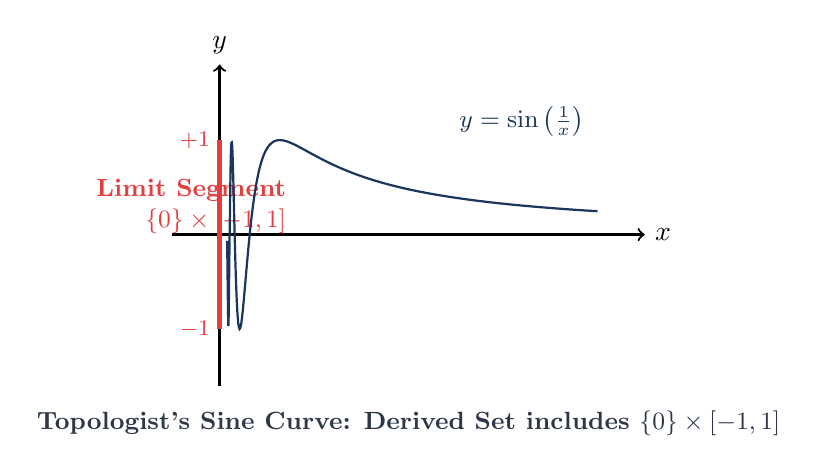
\begin{tikzpicture}[scale=1.2]
    % Topologist's Sine Curve
    \draw[->,thick] (-0.5,0) -- (4.5,0) node[right] {$x$};
    \draw[->,thick] (0,-1.6) -- (0,1.8) node[above] {$y$};
    
    % The limit vertical segment {0} x [-1, 1]
    \draw[ultra thick,crimsonred] (0,-1) -- (0,1);
    \node[crimsonred,font=\bfseries\footnotesize,left] at (0,1) {$+1$};
    \node[crimsonred,font=\bfseries\footnotesize,left] at (0,-1) {$-1$};
    \node[crimsonred,font=\bfseries\small,align=right] at (-0.3,0.3) {Limit Segment\\$\{0\} \times [-1, 1]$};

    % Curve y = sin(1/x)
    \draw[thick,primarynavy,smooth,samples=300,domain=0.08:4] plot (\x,{sin((1/\x)*180/pi)});
    \node[primarynavy,font=\bfseries\small] at (3.2,1.2) {$y = \sin\left(\frac{1}{x}\right)$};

    \node[darkslate,font=\bfseries\small] at (2.0,-2.0) {Topologist's Sine Curve: Derived Set includes $\{0\} \times [-1, 1]$};
\end{tikzpicture}
\end{center}

\newpage

\subsection{Closed Sets in a Metric Space}

\begin{defbox}{Definition: Closed Set}
Let $(X, d)$ be a metric space. A subset $F \subseteq X$ is called a \textbf{closed set} if and only if its complement $F^c = X \setminus F$ is an open set in $(X, d)$.
\end{defbox}

\begin{exbox}{Examples of Closed Sets}
\begin{enumerate}
    \item \textbf{Singleton Sets in $(\mathbb{R}, |\cdot|)$:}
    For any $x \in \mathbb{R}$, the singleton $\{x\}$ is closed because its complement:
    $$\{x\}^c = (-\infty, x) \cup (x, \infty)$$
    is the union of two open intervals (open sets), hence open. Thus, \textbf{every singleton set in a metric space is closed}.
    
    \item \textbf{Closed Intervals in $(\mathbb{R}, |\cdot|)$:}
    $[a, b]$ is closed because $[a, b]^c = (-\infty, a) \cup (b, \infty)$ is open.
\end{enumerate}
\end{exbox}

\subsection{Topological Properties of Closed Sets}

\begin{formulabox}{Duality Properties of Closed Sets (De Morgan's Laws)}
\begin{enumerate}
    \item The empty set $\emptyset$ and the whole space $X$ are \textbf{closed sets} (since $\emptyset^c = X$ and $X^c = \emptyset$ are open).
    \item The \textbf{intersection of an arbitrary collection} of closed sets is closed:
    $$\left( \bigcap_{\lambda \in \Lambda} F_\lambda \right)^c = \bigcup_{\lambda \in \Lambda} F_\lambda^c \quad \text{(Union of open sets is open)}$$
    \item The \textbf{union of a finite number} of closed sets is closed:
    $$\left( \bigcup_{i=1}^n F_i \right)^c = \bigcap_{i=1}^n F_i^c \quad \text{(Finite intersection of open sets is open)}$$
\end{enumerate}
\end{formulabox}

\subsection{Theorem: Limit Point Characterization of Closed Sets}

\begin{exbox}{Theorem: Closed Sets Contain All Their Limit Points}
\textbf{Theorem:} In a metric space $(X, d)$, a subset $F \subseteq X$ is closed if and only if $F$ contains all its limit points ($F' \subseteq F$).

\textbf{Proof:}
\begin{enumerate}
    \item \textbf{($\implies$) Necessary Condition:} Assume $F$ is closed. We must show $F' \subseteq F$.
    \begin{itemize}
        \item Let $p \in F^c = X \setminus F$.
        \item Since $F$ is closed, $F^c$ is an open set.
        \item By definition of an open set, there exists an open ball $S_r(p)$ such that $S_r(p) \subseteq F^c = X \setminus F$.
        \item This implies $S_r(p) \cap F = \emptyset \implies (S_r(p) \setminus \{p\}) \cap F = \emptyset$.
        \item Therefore, $p$ is \textbf{not} a limit point of $F$ ($p \notin F'$).
        \item By contrapositive, if $p \in F'$, then $p \in F$. Thus $F' \subseteq F$.
    \end{itemize}
    
    \item \textbf{($\impliedby$) Sufficient Condition:} Assume $F' \subseteq F$. We must show $F$ is closed (i.e., $F^c$ is open).
    \begin{itemize}
        \item Let $x \in F^c = X \setminus F$.
        \item Since $F' \subseteq F$, we have $x \notin F'$.
        \item Since $x$ is not a limit point of $F$, there exists an open sphere $S_r(x)$ such that:
        $$(S_r(x) \setminus \{x\}) \cap F = \emptyset$$
        \item Since $x \notin F$, we have $S_r(x) \cap F = \emptyset$, which implies $S_r(x) \subseteq X \setminus F = F^c$.
        \item Since $x \in F^c$ was arbitrary, every point of $F^c$ is an interior point of $F^c$.
        \item Thus $F^c$ is open, which proves that $F$ is \textbf{closed}. \qed
    \end{itemize}
\end{enumerate}
\end{exbox}

\newpage

\section{Module 6: Master Quick Revision Cheat Sheet}

\begin{formulabox}{1. Metric Axioms, Norms, and Standard Metrics}
\begin{itemize}
    \item \textbf{Metric Space Axioms $(X, d)$:} $\forall x, y, z \in X$:
    \begin{enumerate}
        \item \textbf{Non-negativity:} $d(x, y) \ge 0$.
        \item \textbf{Identity of Indiscernibles:} $d(x, y) = 0 \iff x = y$.
        \item \textbf{Symmetry:} $d(x, y) = d(y, x)$.
        \item \textbf{Triangle Inequality:} $d(x, z) \le d(x, y) + d(y, z)$.
    \end{enumerate}
    \item \textbf{Standard Metrics on $\mathbb{R}^n$:}
    \begin{itemize}
        \item Euclidean Metric ($L_2$): $d_2(x, y) = \sqrt{\sum_{i=1}^n (x_i - y_i)^2}$
        \item Taxicab / Manhattan Metric ($L_1$): $d_1(x, y) = \sum_{i=1}^n |x_i - y_i|$
        \item Maximum / Chebyshev Metric ($L_\infty$): $d_\infty(x, y) = \max_{1 \le i \le n} |x_i - y_i|$
        \item Discrete Metric on any set $X$: $d(x, y) = 0$ if $x = y$, and $d(x, y) = 1$ if $x \neq y$.
        \item Semi-metric (Pseudo-metric): Satisfies non-negativity, symmetry, and triangle inequality, but $d(x, y) = 0$ is possible for distinct points $x \neq y$ (e.g., $d(x, y) = |x^2 - y^2|$ on $\mathbb{R}$).
    \end{itemize}
    \item \textbf{Matrix Frobenius Norm on $M_{m \times n}(\mathbb{R})$:}
    \begin{equation*}
        d(A, B) = \|A - B\|_F = \sqrt{\sum_{i=1}^m \sum_{j=1}^n (a_{ij} - b_{ij})^2} = \sqrt{\operatorname{Tr}((A - B)^T (A - B))}
    \end{equation*}
\end{itemize}
\end{formulabox}

\vspace{0.2cm}

\begin{defbox}{2. Open Sets, Spheres, and Neighborhoods}
\begin{itemize}
    \item \textbf{Open Sphere (Ball):} $S_r(x_0) = B(x_0, r) = \{x \in X \mid d(x, x_0) < r\}$.
    \item \textbf{Closed Sphere (Ball):} $\overline{S}_r(x_0) = \{x \in X \mid d(x, x_0) \le r\}$.
    \item \textbf{Interior Point:} $x \in A$ is an interior point of $A$ if $\exists r > 0$ such that $S_r(x) \subseteq A$.
    \item \textbf{Open Set:} $A \subseteq X$ is open if every point of $A$ is an interior point of $A$ (i.e., $A = A^\circ$).
    \item \textbf{Fundamental Theorem on Open Balls:} Every open sphere $S_r(x_0)$ in a metric space is an \textbf{open set}.
    \begin{itemize}
        \item Proof radius choice: For any $x \in S_r(x_0)$, choose radius $\mathbf{\rho = r - d(x, x_0) > 0}$, then $S_\rho(x) \subseteq S_r(x_0)$.
    \end{itemize}
    \item \textbf{Topological Properties of Open Sets:}
    \begin{itemize}
        \item $\emptyset$ and $X$ are open sets.
        \item The \textbf{arbitrary union} of open sets is open: $\bigcup_{\lambda \in \Lambda} U_\lambda$ is open.
        \item The \textbf{finite intersection} of open sets is open: $\bigcap_{i=1}^n U_i$ is open.
        \item Infinite intersections of open sets need not be open (Counterexample: $\bigcap_{n=1}^\infty \left(-\frac{1}{n}, \frac{1}{n}\right) = \{0\}$, which is not open in $\mathbb{R}$).
    \end{itemize}
\end{itemize}
\end{defbox}

\newpage

\begin{exbox}{3. Limit Points, Derived Sets, and Closed Sets}
\begin{itemize}
    \item \textbf{Limit Point (Accumulation Point):} A point $p \in X$ is a limit point of $A \subseteq X$ if every open sphere centered at $p$ contains at least one point of $A$ distinct from $p$:
    \begin{equation*}
        \forall r > 0, \quad (S_r(p) \setminus \{p\}) \cap A \neq \emptyset
    \end{equation*}
    (Note: $p$ need not belong to $A$).
    \item \textbf{Derived Set $A'$:} The set of all limit points of $A$.
    \begin{itemize}
        \item For $A = (a, b) \implies A' = [a, b]$.
        \item For Harmonic Set $A = \{1/n \mid n \in \mathbb{N}\} \implies A' = \{0\}$.
        \item For $A = \mathbb{Q} \implies A' = \mathbb{R}$.
        \item For $A = \mathbb{Z} \implies A' = \emptyset$.
    \end{itemize}
    \item \textbf{Isolated Point:} A point $x \in A$ which is \textbf{not} a limit point of $A$ ($\exists r > 0$ such that $S_r(x) \cap A = \{x\}$).
    \item \textbf{Closed Set:} A subset $F \subseteq X$ is closed if its complement $F^c = X \setminus F$ is an open set.
    \item \textbf{Theorem (Limit Point Characterization):} $F \subseteq X$ is closed if and only if $F$ contains all its limit points:
    \begin{equation*}
        \mathbf{F \text{ is closed} \iff F' \subseteq F}
    \end{equation*}
    \item \textbf{Closure of a Set $\overline{A}$:} $\overline{A} = A \cup A'$. $\overline{A}$ is the smallest closed set containing $A$.
    \item \textbf{Topological Properties of Closed Sets:}
    \begin{itemize}
        \item $\emptyset$ and $X$ are closed sets.
        \item The \textbf{arbitrary intersection} of closed sets is closed: $\bigcap_{\lambda \in \Lambda} F_\lambda$ is closed.
        \item The \textbf{finite union} of closed sets is closed: $\bigcup_{i=1}^n F_i$ is closed.
    \end{itemize}
\end{itemize}
\end{exbox}

\end{document}
